%
% Tutorial -- Biasing a BJT Transistor
%
% Copyright (C) 2005 Thierry SCORDILIS <thierry.scordilis@free.fr>
%
% Permission is granted to copy, distribute and/or modify this document
% under the terms of the GNU Free Documentation License, Version 1.1
% or any later version published by the Free Software Foundation.
%

\tutsection{Graphical methods}
You can bias a bipolar junction transistor in several ways. Determining the best method for your application is easy with a graphical technique.

Biasing an active device, such as a bipolar junction transistor (BJT), requires that you set the dc voltages and currents of the device. To optimize the desired result, you need various bias values. For instance, the input de-vice for a low-noise amplifier may have its best noise performance at 50 $\micro\ampere$ of collector current and a maximum of 5V of collector-to-emitter voltage, whereas later amplifier stages may require 20-mA collector current and 18V collector-to-emitter voltage to generate the necessary ac voltage at the output. When you determine the desired bias conditions, you also need to make sure they are repeatable--within certain limits--to ensure consistent performance.

\begin{figure}[htbp]
\begin{center}
	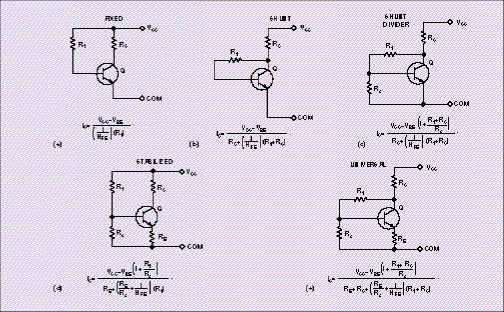
\includegraphics[angle=0,width=0.9\linewidth]{schema}
	\caption{Different feed back technics}
	\label{design:bjt:bias:schemas}
\end{center}
\end{figure}

Biasing-technique analysis for BJTs generally progresses in complexity from the fixed-bias method (see fig \ref{design:bjt:bias:schemas}, to the shunt circuit, to the stabilized circuit, . Studies do not usually cover the shunt-divider  and universal  circuit. However, questions still arise about the bias stability of the shunt bias circuit. It is usable in some noncritical applications, but how inferior is it to the stabilized circuit? Designers are generally taught that the stabilized circuit is the one to use for repeatable biasing.

\bigskip

One way to analyze the stability of the various biasing methods is to use stability factors, which characterize the change in collector current due to changes in the transistor's HFE (current gain), ICBO (collector-to-base leakage current), and VBE . Although these factors are useful, comparing bias circuits and bias-resistor values requires tedious calculations. A visual presentation that compares the stability of the various circuits is more useful.

Looking at the equation for IC in Figure 1b, note that much of the change in IC is due to the differing voltages developed across R1 because of the range of HFE. This difference leads to a question: If some of the current through R1 is fixed, would the result be less voltage change across R1 and hence, less change in IC? This thinking leads to the shunt-divider circuit (Figure 1c). Because VBE changes little, R2 supplies a relatively fixed component of the current through R1, making R1 a smaller value than it would be without R2. The equation for the shunt divider shows that a smaller value of R1 in the denominator causes less change in IC due to changes in HFE. However, along with RC and R2, R1 shows up in the numerator as a multiplying factor for VBE.

\bigskip

You can next look at how strongly each of these factors influences IC. Because you can derive all the circuits in Figure 1 from the universal circuit (Figure 1e) by making the appropriate resistors either infinite (open circuits) or zero (short circuits), the same universality is possible for the equations. Considering the circuit equations and a range of parameters and bias-resistor values, you can produce graphs in which the Y axis represents the change in IC.

To make valid comparisons of the circuits, you need a common parameter related to the biasing for the X axis. The ratio of the collector current to the bias current in R1 works. This ratio is common to the circuits and reflects how stiff the biasing is. To show realistic conditions, the data also includes temperature effects on VBE and HFE for a temperature range of 25 to 75$\degree$C and a 3-to-1 spread in HFE.

For comparison purposes, all the circuits use a 10V supply for VCC at a nominal collector current of 1 mA, with HFE of 100 and VBE of 0.60V at 25$\degree$C. Calculating resistors for 5V VCE and selecting RE to develop 1V at the emitter produces the results for the graphical technique. The model for temperature effects of the device is VBE=0.60?0.002?(T(actual) 25$\degree$C), representing the standard 2-mV/$\degree$C coefficient for diodes. Calculations from the data sheet of the 2N2222A transistor produce an average temperature coefficient for HFE of about 0.58\% /$\degree$C, which you can represent by 

\begin{equation}
HFE_{Temp} =  HFE_{Max}  \times [1+(T(actual)?25\degree C)0.0058] 
\end{equation}

 Calculating IC for a minimum $HFE=50$ at 25$\degree$C and for the maximum $HFE=150$ at 75$\degree$C yields an $HFE_{Temp}$ of 194 and VBE of 0.50V.

This analysis ignores the effects of ICBO. For the nominal collector current of 1 mA and a maximum temperature of 75$\degree$C, the contribution of ICBO to IC is a few percent, at most, for the fixed-bias and shunt-bias circuits in Figures 1a and 1b and less for the bias circuits of Figures 1c, 1d, and 1e.

\tutsubsection{Graphical approach shows trade-offs}

The results of this analysis appear as a simple visual comparison of the current stability of the various types of bias circuits (Figure \ref{design:bjt:bias:curve}). Using this figure, you can select the type of bias circuit and the bias ratios for the necessary stability.

\begin{figure}[htbp]
\begin{center}
	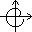
\includegraphics[scale=0.9]{curve}
	\caption{You can compare the performance of the BJT bias circuit by graphing the change in collector current vs the ratio of the collector current to the current in $R1$.}
	\label{design:bjt:bias:curve}
\end{center}
\end{figure}


The horizontal axis is the ratio of the collector current, IC, to the current in resistor R1. This bias ratio applies to all the circuits and indicates how much current is in the base-biasing network compared with the collector current. Thus, a ratio of 1 indicates a stiff bias circuit, with as much current in R1 of the bias network as in the collector, whereas a ratio of 50 indicates that the collector current is 50 times the current in R1 of the bias network. Because some of the results are unexpected, they give renewed consideration to some of the bias circuits previously ignored.

\begin{figure}[htbp]
\begin{center}
	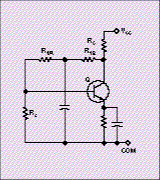
\includegraphics[scale=0.9]{universal}
	\caption{To eliminate the ac effects of feedback, split $R1$, and bypass the center to ground.}
	\label{design:bjt:bias:universal}
\end{center}
\end{figure}

The universal-bias method is obviously the best of the group. The price you pay for its dc stability is the reduction in ac input resistance due to the negative feedback on R1, a sort of Miller effect on resistors. R1 reduces by a factor of the voltage gain plus 1. This feedback may improve distortion and bandwidth as well as reduce the output impedance at the collector. If you don't want these ac effects of feedback, you can eliminate them by splitting R1 into two parts and bypassing the center to ground (Figure \ref{design:bjt:bias:universal}). You can improve performance of this circuit at any bias ratio by increasing the voltage drop across RE, increasing the voltage drop across the collector resistor, or both.

\bigskip

The stabilized circuit has good stability to bias ratios as high as about 12. Above this ratio, its stability rapidly decreases. The stabilized circuit relies on the voltage changes fed back by the emitter current through RE, compared with the voltage, VB, at the base. When the bias ratio becomes less stiff, changes in base current flowing through R1 due to changes in HFE cause significant variations in VB. These variations result in changes in IE and IC. As with the universal circuit, you can improve performance of the stabilized circuit at any bias ratio by increasing the voltage drop across RE. Keep in mind that these results are for a nominal HFE range of 50 to 150 plus temperature effects. Lower minimum values of HFE require stiffer bias ratios for the same performance.

\bigskip

The superior performance of the shunt-divider circuit at bias ratios greater than 12, compared with that of the stabilized circuit, is a surprise. When the shunt-divider circuit's bias is stiff, VC is strongly influenced by the ratio of R1 to R2 times VBE. As VBE changes because of temperature, VC and, thus, IC, change approximately as the ratio of R1 to R2 times VBE changes.

\bigskip
Because IC plays the major role in determining VC, IC experiences wide variations for these stiff biasing ratios. As the ratio becomes less stiff, the changes in VBE with temperature, multiplied by the voltage-divider action, become less dominant, and performance improves until, at the ratio of about 12, the shunt divider's stability starts to surpass that of the stabilized circuit. You can account for this performance by the negative feedback from the collector resistor through R1. Because the collector resistor is usually much larger than the emitter resistor of the stabilized circuit, the stability of the universal circuit holds up better for less stiff bias ratios.

\bigskip
Because the shunt-divider circuit is more stable than the shunt circuit, consider the divider circuit for applications that need less stability than the stabilized or universal circuits offer. Because it saves the cost of the emitter-bypass capacitor necessary in the universal and stabilized circuits, the shunt divider can be more cost-effective. Negative feedback through R1 in the shunt-divider circuit reduces the input resistance and may improve distortion and bandwidth, as well as reduce the output impedance in the same manner as in the universal circuit. Again, you can negate these effects with a bypass capacitor in the center of R1. This bypass capacitor is typically much smaller than the emitter-bypass capacitor for the stabilized circuit.

\bigskip
Because the bias current for the shunt-bias circuit consists of only the base current, it has only one ratio of IC to IR1, namely HFE, and is plotted as a single point. As the bias ratio for the universal and shunt-divider circuits increases, the value of R2 increases until it becomes infinite at an HFE of 100. Under these conditions, the circuits' bias ratios converge with the shunt-circuit ratio.

\bigskip
Figure \ref{design:bjt:bias:curve} leads you to several general conclusions. The universal circuit has the best stability over the widest range of bias ratios. The stabilized circuit has good stability for stiff bias ratios, but you should take care if biasing ratios exceed 12. And, finally, the shunt-divider circuit is a significant improvement over the shunt circuit and is better than the stabilized circuit for large bias ratios.


\tutsection{Simulation technics}
The previous section deals with a graphical method, but a more common method can be to use the simulators to determine all the possible variation for a given schematic ( include $h_{FE}$, Temperature, Voltage regulation, and so on ... ) ; so the problem is more waht kind of feedback I can use or not. Sorry but there is no striaght ansyert since this could a cost issu e for example, or a performance issue\footnote{This point is obviously not understood in the same way when discussing with marketing or development or research teams, who knows why ?}.

\bigskip

Anyway we need to evaluate the different biasing technics using the simulation tool. One analysis will be done in the PA design chapter.
